\documentclass{standalone}
\usepackage{pgfplots}
\pgfplotsset{compat=1.8}
\usepackage{mathtools}
\usepackage{tikz}
\begin{document} 

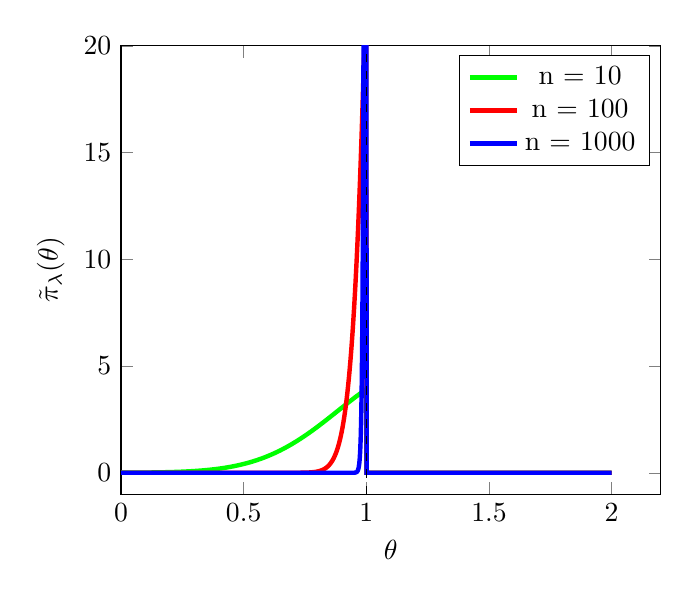
\begin{tikzpicture}
 \begin{axis}[
   scaled ticks=false,
   xmin=0,
   ymin=-1,
   ymax=20,
   xlabel= $\theta$,
   ylabel= $\tilde{\pi}_{\lambda}(\theta)$,
   ]
    \addplot[domain=0:2, green,ultra thick, samples= 1000] {
     4.78* exp(-10*(x-1.2)^2/2)  * (x<1)
    };

  \addplot[domain=0:2, red,ultra thick, samples= 1000] {
     175* exp(-100*(x-1.2)^2/2) * (x<1)
    };

    \addplot[domain=0:2, blue, ultra thick, samples= 1000] {
     100000000000* exp(-1000*(x-1.2)^2/2) * (x<1)
   };

          \addplot +[mark=none, dashed] coordinates {(1, -1) (1, 20)};
  \addlegendentry{n = 10}
\addlegendentry{n = 100}
\addlegendentry{n = 1000}
\end{axis}
\end{tikzpicture}
\end{document}